% ============================================================================
% Paper 2 (plain-language rewrite, three reviews integrated).
% Framing: finite-budget, stated plainly (decoupled > shared under a fixed budget;
% they converge in the limit). No "gated / artifact / allocation-as-slogan".
% Math: GPCM-honest (binary form labeled special case; GPCM forms in appendix);
% free-table = rank up to gauge, for (alpha,beta), with the oracle for "not info";
% link map = exact rank-invariance + local rate-rescale (no "one trajectory");
% rate law = eigenmode + named assumptions; no-kappa leads with the fixed-K test.
% Psychometric: beta = step thresholds; affirm classical IRT; add a magnitude
% (linking-slope) diagnostic so "attenuated" is measured.
% NUMBERS: trajectory/gradient/dynamic/LayerNorm at >=10 seeds (live loss path);
% the neural-IRT oracle, static-code number, magnitude slope, and >=10-seed gate/
% geometry/non-IRT toy are being refreshed by a re-run (slots marked % REFRESH).
% Figures in paper2_figs/. Swap preamble for aaai2026/EDM and thebibliography for
% \bibliography{ref.bib} on Overleaf.
% ----------------------------------------------------------------------------
% REORG (this draft): sections mapped to the target outline (1 Introduction,
% 2 Background, 3 Method, 4.1-4.8 Experiments, 5 Boundaries, 6 Discussion,
% 7 Conclusion, Appendix A-C). GPCM content, experiments, and figures preserved.
% Added the nominal response model (NRM) control in Method and Section 4.5, written
% from deep_irt/bench/outputs/_nrm_sweep.json, _nrm_asym.json, _nrm_ednet_ot.json,
% _nrm_ednet_cov.json and the workshop deck. Classical cross-calibration (4.6) and
% downstream utility (4.7) are marked PLACEHOLDER (specs only, no numbers). Two
% related-work citations carry [VERIFY] footnotes to confirm before submission.
% ============================================================================
\documentclass[twocolumn,10pt]{article}
\usepackage[letterpaper,margin=0.78in]{geometry}
\usepackage{times}
\usepackage{microtype}
\usepackage{amsmath,amssymb}
\usepackage{graphicx}
\usepackage{booktabs}
\usepackage[hyphens]{url}
\usepackage[numbers]{natbib}
\graphicspath{{paper2_figs/}}
\frenchspacing
\setlength{\parskip}{0pt}

\title{\vspace{-2em}Representation Sharing Limits Discrimination Recovery\\
in Amortized Neural IRT}
\author{Wenrui Yuan}
\date{}

\begin{document}
\maketitle

\begin{abstract}
Amortized neural item response theory (IRT) trains an encoder to predict responses and
reads item discrimination and step thresholds from learned representations. The model
predicts well but recovers its parameters at different rates: step thresholds and ability
quickly, discrimination slowly and with high variance across random seeds. We show that
this difference depends on how the representation is arranged. When discrimination is read
from a representation shared with the higher-leverage parameters, it is recovered less accurately
than when it is read from its own representation, although the responses contain enough
information to recover it: a per-item estimator given the true ability recovers
discrimination well. Under a fixed training budget, a decoupled representation, or one
that lets discrimination depend on the inferred ability, recovers discrimination more
accurately than a shared one. The difference shrinks as data and training grow and disappears in the
limit. The effect is specific to discrimination, it is visible in the geometry of the
shared representation, where discrimination occupies about a tenth of the variance while
the step thresholds dominate, and it appears in a non-psychometric encoder as well, so it
is a property of amortized encoders rather than of IRT.
A nominal response control, whose slope on ability carries information comparable to its
intercept, separates two causes the partial credit model ties together. The sharing
trade-off and its decoupling remedy recur for that slope, so they follow from sharing a
representation rather than from low information, while conditioning the readout on the
inferred ability helps only the low-information parameter.
For practice, item discrimination read from a shared representation should be reported
only after the discrimination readout is decoupled.
\end{abstract}

\section{Introduction}
A single neural encoder now serves two purposes in educational measurement. It reads a
learner's response history and predicts the next response, the task on which deep
knowledge tracing is built \citep{piech2015,zhang2017}, and, in neural IRT, it also
exposes interpretable parameters, so the same forward pass returns a learner's ability and
an item's step thresholds and discrimination \citep{yeung2019,wu2020}. The second purpose
is the demanding one. The parameters are meant to be recovered, in the sense that the
recovered values rank items as the true values do, and prediction accuracy does not
guarantee this.

Recovery is in fact uneven. Trained only to predict, an amortized neural IRT model
recovers step thresholds and ability quickly and well, and discrimination slowly,
incompletely, and with large variance across random seeds. A model can rank items by
difficulty correctly and rank them by discrimination poorly while predicting responses
equally well in both cases. The question is why one of the three parameters, read by the
same network from the same responses, is the one left behind.

A rate argument explains part of this. In gradient training the directions with the most
leverage on the loss move first \citep{saxe2014,rahaman2019}, and IRT makes leverage
explicit. The sensitivity of the prediction to discrimination is $\partial p/\partial\alpha
= (\theta-\beta)\,w$ with $w=p(1-p)$, which is zero exactly where the response weight $w$
is largest, near $\theta=\beta$; the sensitivity to ability is $\partial p/\partial\theta =
\alpha\,w$. Discrimination is the low-leverage parameter, so it is learned last. This is
correct and it is incomplete. It concerns a parameter on its own, it predicts a slower
rate rather than a recovery that settles below what the responses allow, and it says
nothing about the item embedding that actually carries discrimination, which the discrimination and
step-threshold heads both read and which also feeds the encoder.

That representation is the subject of this paper. We show that, at the training budgets
used in practice, discrimination is recovered better when it is read from its own
representation than when it shares one with the higher-leverage parameters, and that the
difference is not caused by a shortage of information. Three results establish this. A
per-item estimator given the true ability recovers discrimination from the same responses,
so the responses are informative enough. Holding the responses, the true parameters, and
their information fixed, and changing only whether the representation is shared, changes
how well discrimination is recovered. And the shared representation carries a measurable
trace of the difference: discrimination occupies a small fraction of its variance while
the step thresholds occupy most of it. Decoupling the discrimination readout, or letting
it depend on the inferred ability, removes most of the difference, and the difference
shrinks toward zero as data and training grow.

A nominal response control separates two things the partial credit model ties together.
The nominal model gives each response category a slope on ability whose information is not
low, unlike partial-credit discrimination. That slope still pays the shared-width trade-off
and is still rescued by a separate representation, so the sharing effect follows from
sharing a representation, not from low information. Conditioning the readout on the inferred
ability, by contrast, helps the partial-credit discrimination but degrades the nominal
slope, so that remedy is tied to low information.

The same behavior occurs without any IRT content. A non-psychometric sequence model, with
an encoder and a deliberately low-leverage readout, reproduces it, and a variant with no
encoder does not. Neural IRT is the case where leverage is available in closed form, so
the parameter that will be recovered worst is known before training.

\paragraph{Contributions.}
\begin{enumerate}\itemsep1pt
\item At fixed responses and information, whether the representation is shared changes how
well discrimination is recovered, and a per-item estimator given the true ability recovers
what the shared model does not.
\item The shared representation carries little of the discrimination signal, the step
thresholds dominate it, and the higher-leverage parameters do not benefit from a separate
representation.
\item Decoupling and ability-conditioning each improve discrimination recovery while the
high-leverage control does not move, and the improvement survives a regularization control
that removes a separate ability-overfitting effect.
\item A nominal response control separates sharing from information: the sharing trade-off
and its decoupling remedy recur for a slope whose information is not low, while
ability-conditioning helps only the low-information parameter and degrades the slope whose
information is not low.
\item A non-IRT encoder reproduces the effect, and item discrimination read from a shared
representation should be reported only after decoupling the readout.
\end{enumerate}

\section{Background and Related Work}
\textbf{Prediction and recovery in neural IRT.} Deep knowledge tracing models a response
sequence with a recurrent or attention encoder and is evaluated by next-response prediction
\citep{piech2015,zhang2017,pandey2019}. Neural IRT keeps the encoder and adds an
IRT-structured decoder, so the state gives ability while item heads give step thresholds
and discrimination \citep{yeung2019}, and variational and amortized variants estimate item
parameters jointly \citep{wu2020,tsutsumi2024}. The closest architecture precedent trains
an encoder-decoder neural IRT model and reads item parameters from learned
representations \citep{converse2021},\footnote{[VERIFY] Converse, Pu, and Oliveira, AIED
2021 (LNCS 12749), cited here as the closest encoder-decoder neural-IRT architecture
precedent. Confirm the architecture and that it does not separate recovery by parameter or
study the shared representation.} but it does not separate recovery by parameter or examine
the representation. A variational neural IRT model reports the same weaker recovery of
discrimination and attributes it to the variational objective rather than to the loss
curvature \citep{ma2024}.\footnote{[VERIFY] Ma et al.\ 2024 (arXiv:2310.12010), cited here
as reporting weaker discrimination recovery under a variational objective and blaming the
variational gap. Confirm the exact claim before submission; we find the deficit under a
plain prediction loss with no variational gap.} These models are evaluated by prediction;
where they report recovery, they report it for ability, hold discrimination fixed, or read
all parameters from one shared representation without examining how that sharing affects
each parameter. That question is the subject here.

\textbf{Polytomous IRT and Fisher information.} The generalized partial credit model
\citep{vanderlinden1997,embretson2000} describes an item by a discrimination and a vector
of step thresholds, and gives the information available about each parameter in closed
form. Discrimination's information carries a squared lever arm that is small exactly where
the responses are most informative, so discrimination is the parameter with the least
information in this model. The nominal response model \citep{bock1972} instead gives each
category its own slope on ability and intercept, and there the slope on ability has
information comparable to the intercept, which we use as a control. Because the IRT scale is
identified only up to an affine transformation, recovery is measured by rank rather than by
raw magnitude \citep{embretson2000}.

\textbf{The amortization gap.} Amortized inference replaces a per-instance optimization with
a single network, at a measurable cost in quality \citep{kingma2014,cremer2018}. Our result
is the version of that cost that falls on parameter recovery and is uneven across
parameters. The nearest psychometric models amortize item factor analysis
\citep{urban2021} or joint estimation \citep{molenaar2025}; they read all parameters from
one shared representation and report recovery without separating the parameters, which is
what we do here.

\textbf{Shared representations across multiple readouts.} A representation trained for
several readouts of unequal leverage is used unevenly, a known property of multi-task
learning \citep{caruana1997,ruder2017}. The common responses rebalance or project gradients
so one task does not dominate \citep{chen2018,yu2020}, and compatibility analysis predicts
that mismatched co-trained outputs degrade a shared representation \citep{standley2020}. We
use a structural response instead, separating the representation, and we find that the
readout gradients are orthogonal, so the cost is how the shared representation is used
rather than direct gradient conflict. We are not aware of this question studied for the
recovery of interpretable measurement parameters.

\textbf{Learning dynamics.} That recovery follows leverage is consistent with the dynamics
of gradient learning, in which deep linear networks learn modes in order of their singular
value \citep{saxe2014,advani2017}, with spectral and kernel analogs
\citep{rahaman2019,jacot2018}, and the few large eigenvalues of the Hessian correspond to
the high-leverage directions \citep{sagun2017}. Three lenses give the same ordering and we
borrow the ordering rather than a law from any one of them. The natural gradient rescales
updates by the inverse Fisher information, so under ordinary gradient descent the
low-information directions move more slowly \citep{amari1998}. Spectral analyses of learning
recover modes in order of their singular value or frequency \citep{saxe2014,cao2019}. And
many fitted models are sloppy, with a few stiff directions and many soft ones set by the
same curvature \citep{transtrum2015}. These hold in linear or near-optimum regimes; our
setting is feature learning rather than the lazy regime, since the encoder's representation
changes during training \citep{damian2022}, so we take the leverage ordering as motivation
and establish the effect empirically.

\textbf{Inductive bias and probing.} A parameter that is recoverable from the responses but
not recovered by the trained model is consistent with the result that latent factors are
not recovered without an inductive bias \citep{locatello2019}, and that a structural
constraint promotes separation \citep{higgins2017}; our per-item estimator is a probe on
the encoder output \citep{alain2017}.

\section{Method}
\textbf{Model.} An encoder $E_\phi$ reads an interaction sequence and produces a per-learner
ability state $\theta_t$. Each item $j$ has a learned embedding $e_j$ that feeds the encoder and
is read by heads for discrimination $\alpha_j$ and step thresholds $\beta_j$. A GPCM decoder
maps $(\theta_t,\alpha_j,\beta_j)$ to a distribution over ordered categories, and training
minimizes the response-prediction loss; no parameter is a supervised target.

\textbf{Leverage.} For the binary special case ($K=2$), with $z=\alpha(\theta-\beta)$,
$p=\sigma(z)$, and residual $r=p-y$, the per-parameter gradients are $\partial_\theta
L=r\alpha$, $\partial_\beta L=-r\alpha$, $\partial_\alpha L=r(\theta-\beta)$, and the
single-response Fisher informations are $I(\theta)=I(\beta)=\alpha^2 w$ and
$I(\alpha)=(\theta-\beta)^2 w$ with $w=p(1-p)$. The GPCM forms (Appendix~A) replace the
residual by the per-category residual and the lever arm $(\theta-\beta)$ by a
category-weighted version, and reduce to these at $K=2$; in both, the information about
discrimination carries the squared lever arm $(\theta-\beta)^2$, which is smallest where
the response weight $w$ is largest. So on aggregate discrimination has less information than
ability or the step thresholds, and it is identified before training as the parameter
recovered least accurately.

\textbf{A control whose slope is not low information.} To separate the low information of
discrimination from its being a slope read from a shared representation, we add the nominal
response model \citep{bock1972} as a control. It gives each category its own slope on
ability $a_{i,k}$ and intercept $c_{i,k}$, with
$P(Y_i=k\mid\theta)=\mathrm{softmax}_k(a_{i,k}\theta+c_{i,k})$ and per-category residual
$r_k=p_k-y_k$; through the category logit the gradients are $\partial_{a_k}L=r_k\theta$ and
$\partial_{c_k}L=r_k$ (Appendix~B). The slope $a_k$ is the analogue of GPCM discrimination,
a slope on ability, but its information is not low: the $\theta^2$ multiplier averages to
about one for $\theta\sim\mathcal{N}(0,1)$, so $I(a_k)/I(c_k)\approx0.90$ (3 seeds), not the
several-fold gap discrimination has in GPCM. The nominal model holds the representation
arrangement fixed while removing the low information, so we can ask whether the slope lags
for being a slope in a shared representation or for its low information.

\textbf{Arrangements and controls.} Two arrangements are varied on this one model:
\emph{shared} versus \emph{decoupled}, whether discrimination reads $e_j$ or a separate
embedding, and \emph{static} versus \emph{dynamic}, whether discrimination may read the inferred
state. The controls are also changes to this model: a per-item maximum-likelihood
\emph{oracle} given the true ability and no shared embedding, the step thresholds as a
high-leverage control, a \emph{no-encoder} variant, and \emph{LayerNorm} on the encoder.
The nominal response control uses the same shared, decoupled, static, and dynamic
arrangements, and adds two one-sided decouplings that give only the slope, or only the
intercept, its own wide embedding. Recovery is the sign-aligned rank correlation between
recovered and true values, used throughout for the rank claims; magnitude is reported
separately by linking recovered discrimination to the true scale and reporting the
regression slope and RMSE (Section~5).

\textbf{Non-psychometric model.} To separate the arrangement from the IRT task, we use a
sequence model with no IRT content: a recurrent encoder infers a per-instance state, and a
high-leverage location and a low-leverage slope are read from a shared item embedding that also
feeds the encoder, with leverage set by a knob. The same shared-versus-decoupled change and
the same oracle apply.

\textbf{What the theory settles, and its limits.} Three statements, each scoped. First, near
an identifiable, correctly specified optimum, gradient flow linearizes to $\dot\delta=-F\delta$
with $F$ the Fisher information, so each eigenmode of $F$ decays at a rate equal to its
eigenvalue, and discrimination is the small-eigenvalue mode; this is the rate argument, and
it assumes proximity to the optimum and a near-zero-residual fit. Second, when the item
parameters $(\alpha,\beta)$ form a free table that can reach the optimal prediction, every
gradient is linear in the residual and the gradients vanish together, so the optimum
recovers the true ranks up to the affine gauge, for any readout arrangement, which we
confirm numerically; this applies to the item table and not to the encoder's $\theta$.
Together with the oracle, which recovers discrimination from the same finite responses,
this places the finite-budget difference in the training trajectory rather than in the
information the responses carry. Third, any $C^1$ strictly monotone positive link applied to
discrimination preserves the rank of $\alpha$, so the recovered ranks do not depend on the
link; near the optimum it rescales the discrimination learning rate by a constant that a
matched learning rate absorbs, so the choice of smooth positive link is not the cause.

We do not claim a conditioning-number law. When we break the collinearity between the Fisher
conditioning number and the category count, by varying the conditioning number about
$45\times$ at fixed category count, the difference between shared and decoupled is flat, so
it does not track the conditioning number. The difference grows with the category count
through ordinal information, not through conditioning.

\textbf{Protocol.} Responses are generated from a known GPCM ($N=800$, $Q=60$, $T=60$,
$\theta\sim\mathcal{N}(0,1)$, $\alpha\sim\mathrm{LogNormal}(0,0.3)$). The encoder is an LSTM,
and the results replicate on Transformer and DKVMN encoders. Each reported comparison uses
at least ten random seeds with bootstrap confidence intervals and paired across-seed tests,
except the nominal response control (Section~4.5), which uses eight seeds at $K=4$.

\section{Experiments}
% REFRESH: oracle (neural IRT), static-code number, magnitude slope, and >=10-seed gate /
% geometry / non-IRT toy are being updated by the consistency re-run; numbers below are the
% current values pending that refresh.

\subsection{Recovery follows Fisher information}
\begin{figure}[t]\centering
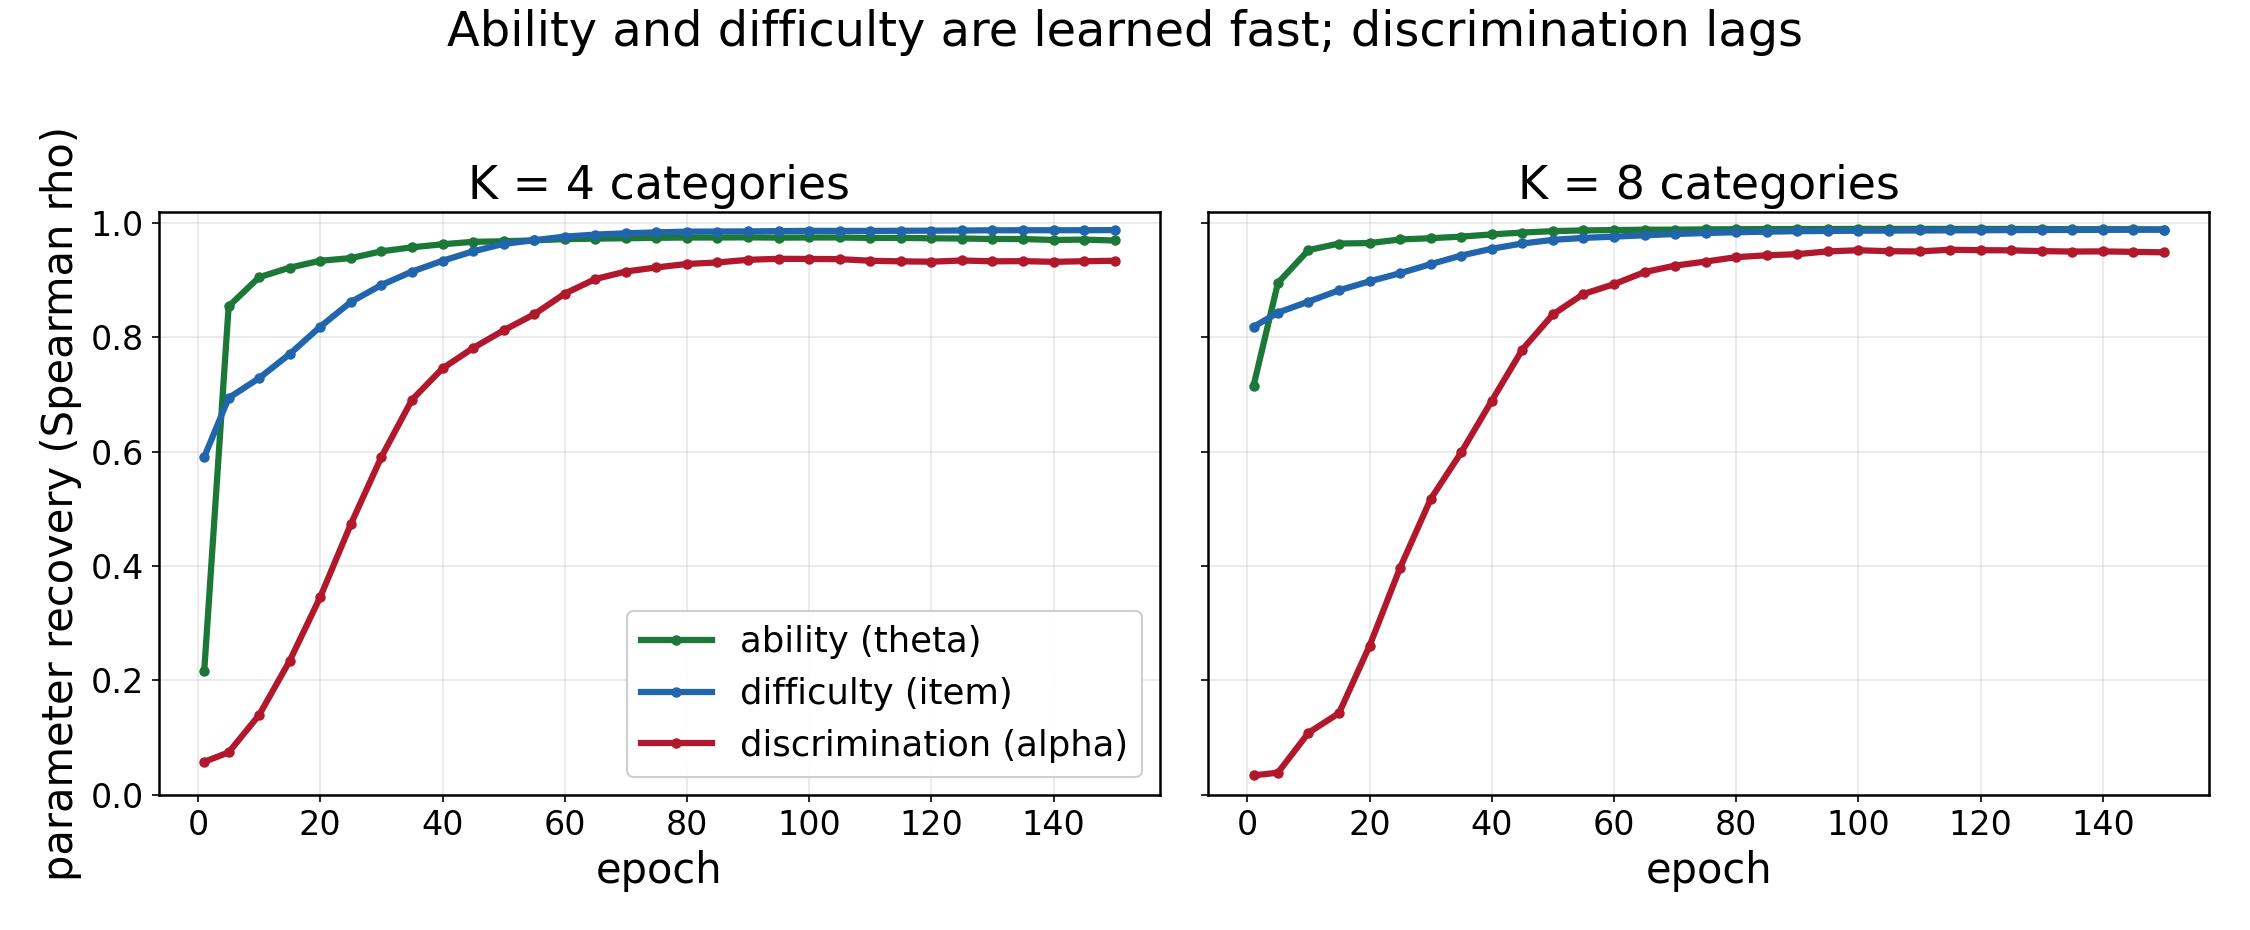
\includegraphics[width=\columnwidth]{s1_three_speeds.png}
\caption{Recovery follows leverage: ability and the step thresholds rise quickly,
discrimination slowly.}
\label{fig:rate}
\end{figure}

The recovery curves match the rate argument (Figure~\ref{fig:rate}): ability and the step
thresholds reach high rank early, and discrimination lags by hundreds of epochs. The rest of
this section asks whether the discrimination lag is set by the information in the responses
or by the representation, and what changes it.

\subsection{The information is sufficient, and the arrangement changes recovery}
\textbf{The responses are informative enough.} If the difference were a shortage of
information, no estimator should recover discrimination from these responses. A per-item
estimator given the true ability does recover it, at $0.83$ where the shared model reaches
$0.55$ at the low-leverage setting of the non-psychometric model (Table~\ref{tab:general}).
% REFRESH: replace with the neural-IRT per-item oracle (shared vs decoupled vs oracle).
The responses carry the discrimination signal, and the shared model does not use all of it.

\begin{table}[t]\centering\small
\begin{tabular}{lcccc}
\toprule
leverage & shared & decoupled & difference & oracle\\
\midrule
high & 0.92 & 0.93 & $+0.01$ & 0.80\\
mid  & 0.85 & 0.89 & $+0.04$ & 0.92\\
\textbf{low} & \textbf{0.55} & \textbf{0.70} & \textbf{+0.15} & \textbf{0.83}\\
\bottomrule
\end{tabular}
\caption{Non-psychometric model: recovery of the low-leverage readout ($|\rho|$, 5 seeds).
The oracle recovers what the shared model does not, and decoupling improves recovery as
leverage falls.}
\label{tab:general}
\end{table}

\textbf{The arrangement changes recovery at fixed data.} If the difference were
representational, changing only the arrangement, with the responses and parameters fixed,
should change recovery. It does. Widening the shared item embedding in neural IRT traces a
trade-off in which ability recovery falls from $0.97$ to $0.88$ as discrimination rises from
$0.66$ to $0.91$, and no width recovers both; a separate embedding recovers ability near $0.97$
and discrimination between $0.90$ and $0.94$ at the same total capacity, and holds this as
capacity grows (Figure~\ref{fig:frontier}). The difference is in how the representation is
used, not in how much of it there is.

\begin{figure}[t]\centering
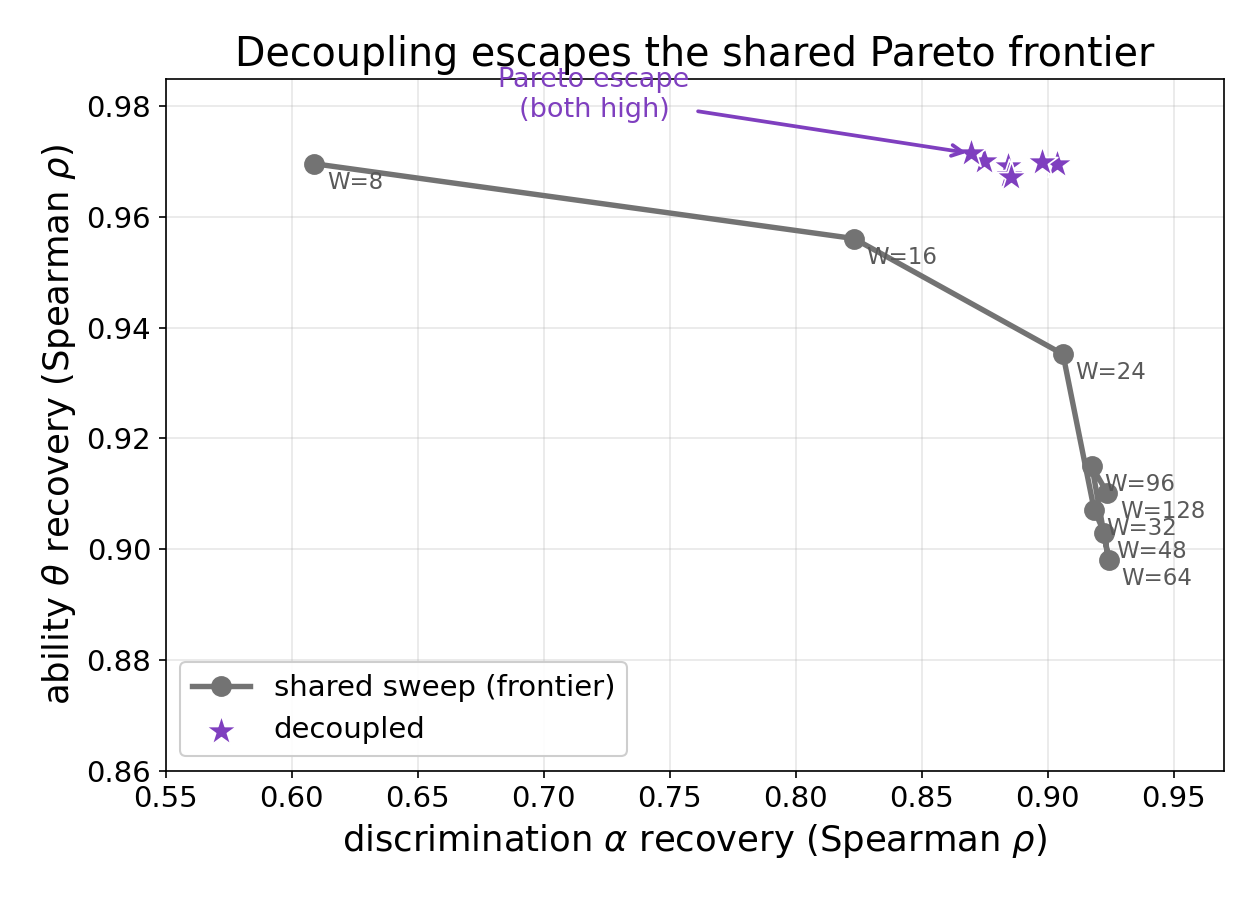
\includegraphics[width=\columnwidth]{j3_tradeoff_frontier.png}
\caption{A shared item embedding trades ability against discrimination as its width
changes; a separate embedding recovers both at the same total capacity.}
\label{fig:frontier}
\end{figure}

\subsection{Geometry of the shared embedding}
\textbf{The shared representation carries little discrimination.} If capacity is spent on
the higher-leverage parameters, discrimination should occupy little of the shared embedding, and
the high-leverage parameters should not benefit from a separate embedding. A linear probe of the
shared item embedding recovers the step thresholds at $R^2=0.96$ and discrimination at $R^2=0.64$,
and discrimination accounts for about $11\%$ of the embedding's variance (Table~\ref{tab:geom});
the step thresholds gain nothing from a separate embedding.

\begin{table}[t]\centering\small
\begin{tabular}{lccc}
\toprule
 & probe $R^2$, $\alpha$ & probe $R^2$, $\beta$ & $\alpha$ var.\ frac.\\
\midrule
shared & 0.64 & 0.96 & 0.115\\
decoupled & -- & 0.86 & 0.013\\
\bottomrule
\end{tabular}
\caption{Geometry of the shared item embedding ($\ge$10 seeds). The step thresholds dominate;
discrimination accounts for about $11\%$ of the variance. The decoupled $\alpha$ probe is
undefined because $\alpha$ no longer lies in the shared embedding.}
\label{tab:geom}
\end{table}

\textbf{Mechanism and controls.} The shared item embedding comes to favor the higher-leverage
parameters during training. Under sharing, discrimination recovery rises to $0.92$ near
epoch~100 and falls to $0.85$ by epoch~500, in all ten seeds and as an internal maximum in
each, while the separate embedding rises and holds (Figure~\ref{fig:traj}). The gradient on the
shared embedding from the ability pathway grows about $30\times$ over training (95\% CI
$[20,43]$) while the discrimination pathway stays flat, and the two are orthogonal (cosine
near zero), so the cost is not direct gradient conflict but the use of the shared embedding for
the higher-leverage parameters, as the geometry above shows. Regularization separates this
from ordinary overfitting: LayerNorm reduces a distinct ability decay (from $-0.18$ to
$-0.06$) but leaves the discrimination rise-and-fall unchanged ($-0.075$ to $-0.074$). The
difference is finite-budget: at a fixed budget it does not shrink as data grow
(Figure~\ref{fig:nsweep}), and it disappears only as data and training grow together. By the
linking slope, shared discrimination is also attenuated in magnitude relative to a decoupled
or per-item estimate. % REFRESH: report linking slope and RMSE, shared vs decoupled vs oracle.

\begin{figure}[t]\centering
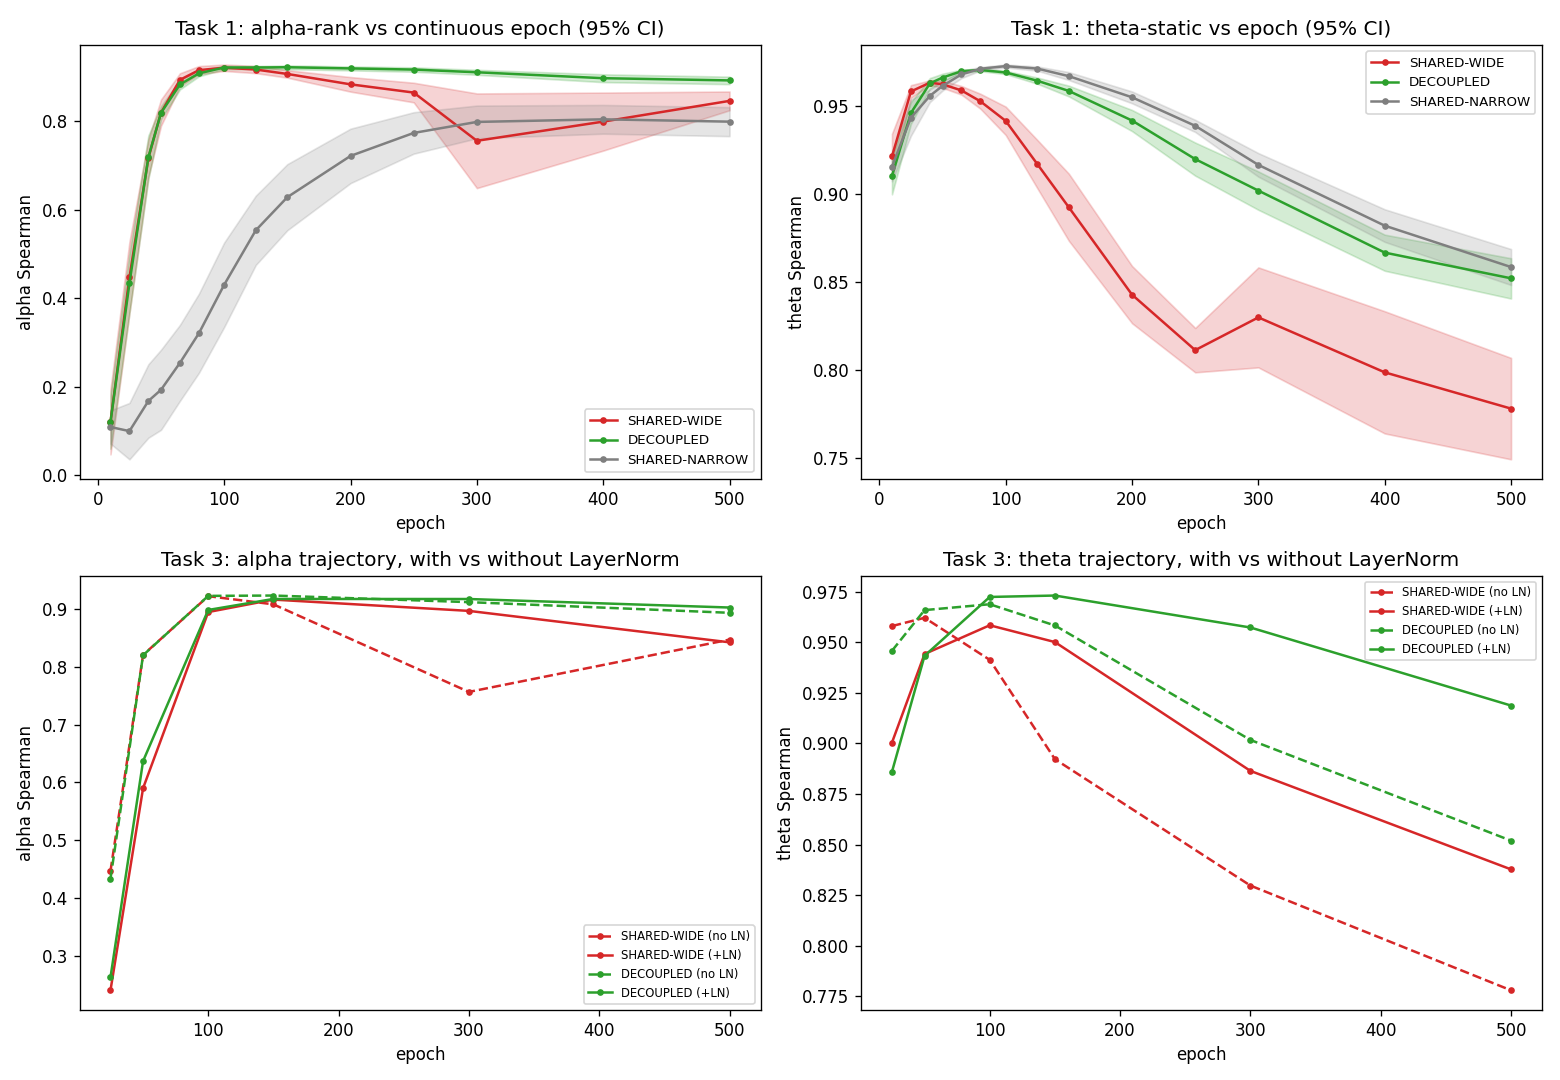
\includegraphics[width=\columnwidth]{rigor_paper2_trajectory.png}
\caption{Discrimination recovery over training (10 seeds, 95\% CI). The shared embedding rises
then falls; the separate embedding holds. LayerNorm removes a separate ability decay but not the
discrimination rise-and-fall.}
\label{fig:traj}
\end{figure}

\begin{figure}[t]\centering
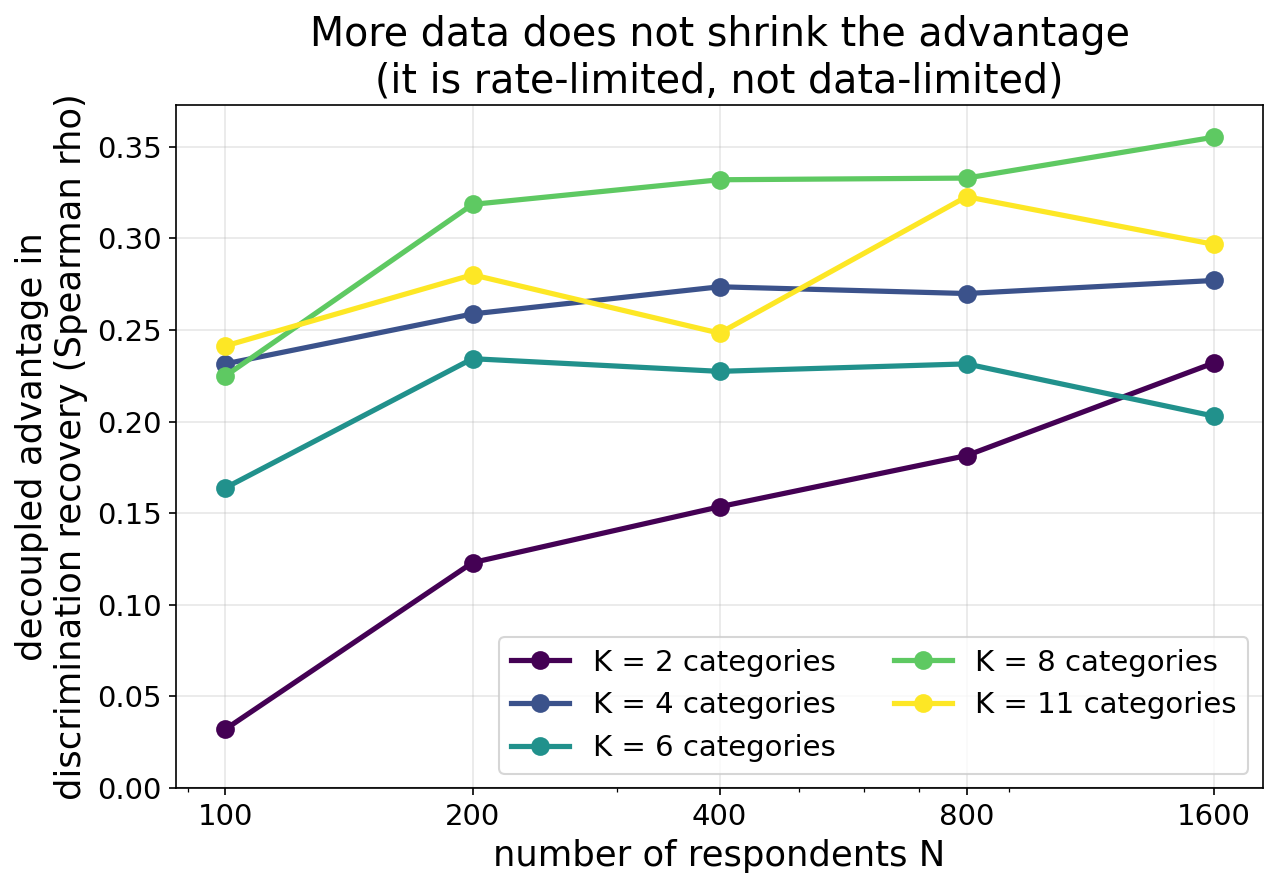
\includegraphics[width=\columnwidth]{d5_finite_sample_Nsweep.png}
\caption{At a fixed training budget the shared-decoupled difference does not shrink as data
grow.}
\label{fig:nsweep}
\end{figure}

\subsection{Interventions and the category count}
\textbf{Two interventions improve recovery, and the control is unaffected.} Giving discrimination its
own embedding is the comparison above. Letting discrimination depend on the inferred ability
improves its recovery for $K\ge4$, by an amount that grows with the number of categories,
significant across twelve seeds (paired Wilcoxon $p\le0.007$, confidence intervals excluding
zero), with no effect at $K=2$ (Table~\ref{tab:dynamic}). The step thresholds, which share
ability's leverage ($I(\beta)=I(\theta)=\alpha^2 w$), are unaffected by either change, so the
improvement is specific to the low-leverage parameter and is not a general effect of added
flexibility.

\begin{table}[t]\centering\small
\begin{tabular}{lccc}
\toprule
$K$ & $\Delta_\alpha$ (95\% CI) & Wilcoxon $p$ & $\Delta_\beta$\\
\midrule
2  & $-0.003$ $[-0.04,+0.03]$ & 0.68   & $+0.000$\\
4  & $+0.032$ $[+0.01,+0.06]$ & 0.005  & $+0.001$\\
8  & $+0.059$ $[+0.03,+0.09]$ & 0.001  & $+0.000$\\
11 & $+0.186$ $[+0.12,+0.25]$ & 0.0005 & $+0.000$\\
\bottomrule
\end{tabular}
\caption{Ability-conditioned versus static discrimination (12 seeds, paired). The
improvement grows with $K$; the step-threshold control is unaffected.}
\label{tab:dynamic}
\end{table}

\subsection{The nominal response dissociation}
The partial credit model ties two properties together, a slope on ability and a low
information, so the discrimination lag could come from either. The nominal response model
separates them: its slope $a_k$ is a slope on ability whose information is not low
($I(a_k)/I(c_k)\approx0.90$). Trained the same way, on $N=800$, $Q=60$, $K=4$, at $150$
epochs over eight seeds, it tells the two apart (Table~\ref{tab:nrm}).

\textbf{The slope is not the slow one.} At a shared width of $8$ the slope and the intercept
recover alike, the slope $a_k$ at $0.85$ and the intercept $c_k$ at $0.89$, and a separate
wide key raises both to $0.980$ and $0.982$. There is no ordering gap of the kind
discrimination shows in GPCM. The lag came from low information, not from being a slope.

\textbf{The shared trade-off is representation.} Widening the shared embedding raises the
slope by $+0.093$ from width $8$ to width $32$ but lowers ability by $-0.177$, the same
trade-off the partial credit model shows, and it appears even though the nominal slope's
information is not low, so it tracks the slope sharing a representation with ability rather
than the information being low. A separate wide key clears it, recovering the slope at
$0.980$, the intercept at $0.982$, and ability at $0.853$, all above the best shared width at
once. Within the nominal model only the intercept needs the wide key: decoupling the
intercept $c_k$ alone leaves the slope at $0.964$ on the narrow value, decoupling the slope
$a_k$ alone drops the intercept to $0.392$, and separate keys for both add nothing
($0.978$ and $0.973$). The intercept carries the wide-key capacity while the slope shares it.

\textbf{Ability-conditioning helps only the low-information parameter.} Conditioning the
readout on the inferred state rescued GPCM discrimination, which has low information, but it
lowers the nominal slope, whose information is not low, from $0.980$ to $0.735$. The
conditioned slope is stable across learner halves, split-half about $0.999$, while its
recovery falls to $0.735$, so where the information is not low the state adds noise rather
than signal. The remedy is tied to low information, not to the sharing.

\begin{table}[t]\centering\small
\begin{tabular}{lccc}
\toprule
arrangement & $a_k$ (slope) & $c_k$ (intercept) & ability\\
\midrule
shared, width 8   & 0.85 & 0.89 & 0.80\\
shared, width 32  & 0.94 & 0.90 & 0.62\\
decoupled (wide key) & \textbf{0.98} & \textbf{0.98} & \textbf{0.85}\\
\quad + dynamic slope & 0.74 & 0.97 & 0.86\\
decouple $c_k$ only  & 0.96 & 0.98 & 0.87\\
decouple $a_k$ only  & 0.87 & 0.39 & 0.81\\
separate keys, both  & 0.98 & 0.97 & 0.84\\
\bottomrule
\end{tabular}
\caption{Nominal response model recovery ($|\rho|$, 8 seeds; $N{=}800$, $Q{=}60$, $K{=}4$,
150 epochs). Widening the shared embedding raises the slope $a_k$ but lowers ability; a
separate wide key recovers slope, intercept, and ability at once. Conditioning the slope on
the inferred state lowers its recovery, although its information is not low. Decoupling the
intercept $c_k$ alone leaves the slope high on the narrow value, while decoupling the slope
alone breaks the intercept, so the intercept carries the wide-key capacity while the slope
shares it.}
\label{tab:nrm}
\end{table}

Two mechanisms are now separated. The shared trade-off and the decoupling escape recur for
the nominal slope, so they are properties of sharing a representation and hold whether or
not the information is low. Conditioning on the inferred ability, by contrast, helps only
where the information is low, so it splits the two models. Discrimination in GPCM has both at
once, low information and a slope sharing the step thresholds' representation; the nominal
slope has only the second.

\subsection{Recovery versus reliability on real data}
On a real corpus there is no ground truth for the item parameters, so we use split-half
reliability, the agreement of a recovered parameter across two random halves of the
learners, as a proxy for recovery. On EdNet and KDD Cup 2010, discrimination is recovered
far less reliably than the step thresholds, EdNet discrimination about $0.79$ against step
thresholds about $0.94$, KDD about $0.63$ against about $0.85$, and it is under-allocated in
the shared embedding, occupying about $1.5\%$ of its variance against the step thresholds'
about $2.5\%$. The dynamic head is again the lever that does not cost prediction: it is at
least as reliable as the static head in every cell and it rescues the thin static decoupled
channel, which otherwise collapses (KDD discrimination reliability about $0.39$), by about
$0.15$ on EdNet and about $0.25$ on KDD. Decoupling alone can hurt on real data; the dynamic
head does not.

\textbf{[PLACEHOLDER: classical cross-calibration]} We will fit a classical GPCM calibration
by marginal maximum likelihood (an EM estimator) on the items with the highest response
counts and use it as an external reference for discrimination, then test whether the
neural-recovered discrimination agrees with it in rank (Spearman) and whether the decoupled
or dynamic configurations agree better than the shared one. The classical calibration
assumes a static ability, so the comparison is restricted to items and windows where that
assumption is defensible, and disagreement that tracks ability change is reported
separately. This turns the real-data claim from reliability alone into agreement with an
external calibration.

On EdNet option tracing, where each interaction records the chosen option and there is again
no ground truth, the decoupling escape depends on coverage. At about twelve observations per
item the escape reverses, with shared ability reliability about $0.68$ above decoupled about
$0.29$. At knowledge-component density, about $845$ observations per unit, it revives, with
decoupled about $0.66$ against shared about $0.70$. The dynamic head does not rescue at that
density, at about $0.49$ below the static about $0.66$. The escape needs coverage; that the
dynamic head still does not help here is the portable finding.

\subsection{Downstream utility}
\textbf{[PLACEHOLDER: downstream utility]} We will run a computerized adaptive testing
simulation that selects each next item by maximum Fisher information at the running ability
estimate, using the recovered discrimination and difficulty from each configuration (shared,
decoupled, static, dynamic) and the per-item oracle as the ceiling, and scores each by the
ability error against the true value at a fixed test length. A companion item-screening test
flags the truly low-discrimination items from the recovered estimates. The simulation will
show whether the more accurately recovered discrimination of the decoupled and dynamic
configurations yields lower ability error or shorter tests, and how far each sits below the
oracle ceiling.

\subsection{The effect is not specific to IRT}
The non-psychometric model reproduces all of this: decoupling improves the low-leverage
readout, the oracle recovers what the shared model does not, the high-leverage readout does
not benefit, and decoupling reduces the across-seed variance (Table~\ref{tab:general}). A
variant with no encoder shows no decoupling benefit, % REFRESH: report the no-encoder number.
which places the effect in the encoder's shared representation rather than in shared readouts
in general. Neural IRT is the case where leverage is available in closed form, so the
parameter that will be recovered worst is known before training.

\section{Boundaries of the Claim}
The evidence for the dynamics is synthetic. On real data we report reliability, the agreement
of a recovered parameter across learner halves, not recovery against externally calibrated
values; a classical cross-calibration is specified but not yet run (Section~4.6), so the
real-data claim is reliability plus a pending calibration, not ground-truth recovery. The
result is a finite-budget difference, not a quantitative law: the dependence on data versus
training differs between the non-psychometric model and neural IRT, and there is no
conditioning-number rate law. The theory is known in parts, the rate argument near the
optimum, the free-parameter-table invariant, and the link invariance, each established
separately, and we present it as a translation of these into the recovery setting rather than
a new dynamics law. We tested and rejected several stronger statements and keep them on
record: the link is not the cause, there is no population-limit dynamics law, the conditioning
number is not the cause, the recovered-discrimination error does not correlate with ability or
step thresholds, and the effect requires the encoder rather than appearing for shared readouts
in general.

\section{Discussion}
The result is the per-parameter form of leverage-ordered learning \citep{saxe2014} and the
parameter-recovery form of the amortization cost \citep{cremer2018}, and it leaves classical
IRT estimation in place: the model is identified and the estimator is consistent, and what
we add is a property of the amortized estimator at finite budgets. It is not gradient
conflict, since the readout gradients are orthogonal; where multi-task methods rebalance
gradients \citep{chen2018,yu2020}, we separate the representation. The separation is
reminiscent of weight normalization, which separates a magnitude from a direction
\citep{salimans2016}, and here it has a known target, since IRT identifies the low-leverage
parameter in advance.

The nominal response control shows these are two separate mechanisms. Sharing a
representation sets the width trade-off and the decoupling remedy, and applies to any slope
read from the shared embedding whether or not its information is low. The information sets
the recovery rate and whether conditioning the readout on the inferred ability helps, which
is why the dynamic head rescues the low-information discrimination of GPCM but degrades the
higher-information slope of the nominal model. Discrimination in GPCM carries both at once, a
low information and a slope sharing the step thresholds' representation; the nominal slope
carries only the second.

For practice the consequence is direct. Discrimination recovered from a shared neural IRT
model is recovered less accurately, less stably across seeds, and attenuated in magnitude;
decoupling the discrimination readout, or conditioning it on the inferred ability, improves
the recovered ranking at no cost to prediction. Because IRT identifies the low-leverage
parameter in advance, the change can be made by design rather than found by trial.

\section{Conclusion}
Trained to predict, an amortized neural IRT model recovers its parameters at different
rates, and discrimination is recovered least accurately, not because the responses are uninformative
but because, at finite training budgets, it is read from a representation shared with the
higher-leverage parameters. The difference is specific to discrimination, it is visible in
the geometry of the shared representation, and it is removed by giving discrimination its
own representation or the inferred ability. A nominal response control separates the two
mechanisms: sharing a representation sets the trade-off and its decoupling remedy for any
slope, while conditioning on the inferred ability helps only the low-information parameter.
The effect appears without IRT content, so it is a property of amortized encoders, and neural
IRT is the case where the affected parameter is known in advance. Item discrimination read
from a shared representation should be reported only after the readout is decoupled.

\appendix
\section{GPCM gradients and information}
For $K$ ordered categories, let $p_k$ be the GPCM category probabilities, $R_k=p_k-y_k$ the
per-category residual, and $B_k=\sum_{c\le k}\beta_c$. The per-parameter gradients are
$\partial_\theta L=\alpha\sum_k R_k\,k$, $\partial_\alpha L=\sum_k R_k(k\theta-B_k)$, and
$\partial_{\beta_c}L=-\alpha\sum_{k\ge c}R_k$, and the single-response Fisher informations
are $I(\theta)=\alpha^2\mathrm{Var}_p(k)$, $I(\alpha)=\mathrm{Var}_p(k\theta-B_k)$, and
$I(\beta_c)=\alpha^2 P_{\ge c}(1-P_{\ge c})$. These reduce to the binary forms in Section~3
at $K=2$, and in all cases the information about discrimination carries the squared
category-weighted lever arm.

\section{Nominal response gradients and information}
The nominal response model gives item $i$ category slopes $a_{i,k}$ and intercepts $c_{i,k}$
with $P(Y_i=k\mid\theta)=\mathrm{softmax}_k(a_{i,k}\theta+c_{i,k})$ and per-category residual
$r_k=p_k-y_k$. Through the category logit $z_k=a_k\theta+c_k$, with $\partial_{a_k}z_k=\theta$
and $\partial_{c_k}z_k=1$, the gradients are $\partial_{a_k}L=r_k\theta$ and
$\partial_{c_k}L=r_k$. The single-response information about a slope carries the factor
$\theta^2$ relative to the matched intercept, so under $\theta\sim\mathcal{N}(0,1)$ the two
informations are comparable in expectation, $\mathbb{E}[\theta^2]=1$; empirically
$I(a_k)/I(c_k)\approx0.90$ across seeds. This is the sense in which the nominal slope is a
slope on ability whose information is not low, unlike GPCM discrimination whose information
carries the squared lever arm $(\theta-\beta)^2$ that is small where the responses
concentrate.

\section{The free-parameter-table invariant and gauge handling}
When the item parameters form a free table that can reach the optimal prediction, every
parameter gradient is linear in the per-category residual, so at the optimum all residuals
and all item gradients vanish together and the recovered item ranks match the true ranks up
to the affine gauge, for any readout arrangement; we confirm this numerically for the item
table. It does not apply to the encoder's $\theta$, which is not a free table. Because the
IRT scale is identified only up to an affine transformation, and any $C^1$ strictly monotone
positive link on discrimination preserves its rank, recovery is measured throughout by the
sign-aligned rank correlation rather than by raw magnitude, and only the single global scale
is non-identifiable. Magnitude, where reported, is obtained by linking the recovered
discrimination to the true scale and reporting the regression slope and RMSE at the optimal
scale, which separates a genuine attenuation from the gauge.

\small
\begin{thebibliography}{46}
\bibitem{piech2015} C.~Piech et al. Deep knowledge tracing. \emph{NeurIPS}, 2015.
\bibitem{zhang2017} J.~Zhang et al. Dynamic key-value memory networks for knowledge tracing.
\emph{WWW}, 2017.
\bibitem{pandey2019} S.~Pandey, G.~Karypis. A self-attentive model for knowledge tracing.
\emph{EDM}, 2019.
\bibitem{yeung2019} C.-K.~Yeung. Deep-IRT: making deep learning based knowledge tracing
interpretable using item response theory. \emph{EDM}, 2019.
\bibitem{wu2020} M.~Wu et al. Variational item response theory. \emph{EDM}, 2020.
\bibitem{tsutsumi2024} E.~Tsutsumi et al. Deep item response theory as a representation of
interpretable knowledge. \emph{IEEE Trans.\ Learning Technologies}, 2024.
\bibitem{converse2021} G.~Converse, S.~Pu, S.~Oliveira. [VERIFY title] Encoder-decoder neural
item response theory. \emph{AIED}, LNCS 12749, 2021.
\bibitem{ma2024} [VERIFY authors, title] Ma et al. Variational neural item response theory.
arXiv:2310.12010, 2024.
\bibitem{vanderlinden1997} W.~van der Linden, R.~Hambleton (eds.). \emph{Handbook of Modern
Item Response Theory} (GPCM, Muraki). Springer, 1997.
\bibitem{bock1972} R.~D.~Bock. Estimating item parameters and latent ability when responses
are scored in two or more nominal categories. \emph{Psychometrika}, 37(1), 1972.
\bibitem{embretson2000} S.~Embretson, S.~Reise. \emph{Item Response Theory for
Psychologists}. Erlbaum, 2000.
\bibitem{kingma2014} D.~Kingma, M.~Welling. Auto-encoding variational Bayes. \emph{ICLR},
2014.
\bibitem{cremer2018} C.~Cremer, X.~Li, D.~Duvenaud. Inference suboptimality in variational
autoencoders. \emph{ICML}, 2018.
\bibitem{urban2021} C.~Urban, D.~Bauer. A deep learning algorithm for high-dimensional
exploratory item factor analysis. \emph{Psychometrika}, 86(1), 2021.
\bibitem{molenaar2025} D.~Molenaar et al. An autoencoder for amortized joint maximum
likelihood estimation in item factor analysis. \emph{Multivariate Behavioral Research},
60(4), 2025.
\bibitem{caruana1997} R.~Caruana. Multitask learning. \emph{Machine Learning}, 28, 1997.
\bibitem{ruder2017} S.~Ruder. An overview of multi-task learning in deep neural networks.
arXiv:1706.05098, 2017.
\bibitem{chen2018} Z.~Chen et al. GradNorm: gradient normalization for adaptive loss
balancing in deep multitask networks. \emph{ICML}, 2018.
\bibitem{yu2020} T.~Yu et al. Gradient surgery for multi-task learning. \emph{NeurIPS}, 2020.
\bibitem{standley2020} T.~Standley et al. Which tasks should be learned together in
multi-task learning? \emph{ICML}, 2020.
\bibitem{saxe2014} A.~Saxe, J.~McClelland, S.~Ganguli. Exact solutions to the nonlinear
dynamics of learning in deep linear neural networks. \emph{ICLR}, 2014.
\bibitem{advani2017} M.~Advani, A.~Saxe. High-dimensional dynamics of generalization error in
neural networks. arXiv:1710.03667, 2017.
\bibitem{amari1998} S.~Amari. Natural gradient works efficiently in learning. \emph{Neural
Computation}, 10(2), 1998.
\bibitem{cao2019} Y.~Cao et al. Towards understanding the spectral bias of deep learning.
arXiv:1912.01198, 2019.
\bibitem{transtrum2015} M.~Transtrum et al. Perspective: sloppiness and emergent theories in
physics, biology, and beyond. \emph{J.\ Chem.\ Phys.}, 143(1), 2015.
\bibitem{rahaman2019} N.~Rahaman et al. On the spectral bias of neural networks. \emph{ICML},
2019.
\bibitem{jacot2018} A.~Jacot, F.~Gabriel, C.~Hongler. Neural tangent kernel. \emph{NeurIPS},
2018.
\bibitem{sagun2017} L.~Sagun et al. Empirical analysis of the Hessian of over-parametrized
neural networks. arXiv:1706.04454, 2017.
\bibitem{damian2022} A.~Damian, J.~Lee, M.~Soltanolkotabi. Neural networks can learn
representations with gradient descent. \emph{COLT}, 2022.
\bibitem{locatello2019} F.~Locatello et al. Challenging common assumptions in the unsupervised
learning of disentangled representations. \emph{ICML}, 2019.
\bibitem{higgins2017} I.~Higgins et al. beta-VAE: learning basic visual concepts with a
constrained variational framework. \emph{ICLR}, 2017.
\bibitem{alain2017} G.~Alain, Y.~Bengio. Understanding intermediate layers using linear
classifier probes. \emph{ICLR Workshop}, 2017.
\bibitem{salimans2016} T.~Salimans, D.~Kingma. Weight normalization. \emph{NeurIPS}, 2016.
\end{thebibliography}

\end{document}
